% cSpell:ignore bibfile

\documentclass{beamer}
	
	% cSpell:disable

% CLI arguments

\newif\ifrelease%

\ifdefined\debug%
	\releasefalse%
\else
	\releasetrue%
\fi


\newif\ifnotes%

\ifdefined\generatenotes%
	\notestrue%
\else
	\notesfalse%
\fi


	local-dev


	% cSpell:disable

\usepackage{appendixnumberbeamer}
\usepackage{pgfpages}
\usepackage{booktabs}
\usepackage{bm}
\usepackage{mathtools}


	% cSpell:disable

\usetheme[
	progressbar=frametitle,
	titleformat section=smallcaps
]{metropolis}

\ifnotes%
	\setbeameroption{show notes on second screen}
\fi

\title{Data-X Talk} % chktex 13

\subtitle{Path ORAM:\ An Extremely Simple Oblivious RAM Protocol~\cite{DBLP:journals/corr/abs-1202-5150}}

\date{Built from \href{https://git.dbogatov.org/bu/PathORAM-Talk/commit/\version}{\emph{\version}} on \today}

\author{Dmytro Bogatov \\ dmytro@bu.edu}

\institute{Boston University}

\logo{
	
\includegraphics[
		width=1cm,
		height=1cm,
		keepaspectratio
	]{static/logo.eps}\hspace{325pt}\vspace{-30pt}
}

\addbibresource{bibfile.bib}

\makeatletter
	\def\beamer@framenotesbegin{% at beginning of slide
		\usebeamercolor[fg]{normal text} 
			\gdef\beamer@noteitems{}%
			\gdef\beamer@notes{}% 
	}
\makeatother

\lstset{
	mathescape=true,
	numbers=left,
	tabsize=4,
	numbersep=10pt,
	breaklines=true,
	showtabs=false,
	morekeywords={for,end,do,while,if,then,else,Applies,when,return,true,false,Action},
	basicstyle=\normalfont,
	columns=fullflexible,
	frame=leftline,
	xleftmargin=15pt,
	escapechar=|
}

\hypersetup{
	pdfcopyright={Copyright (C) Dmytro Bogatov \the\year. Creative Commons Attribution-NoDerivatives 4.0 International.},
	pdflicenseurl={https://creativecommons.org/licenses/by-nd/4.0/legalcode},
	pdfauthor={Dmytro Bogatov},
	pdftitle={Data-X Talk},
	pdfsubject={Path ORAM:\ An Extremely Simple Oblivious RAM Protocol},
	pdfkeywords={Data-X, Talk, ORAM, PathORAM, Oblivious, Security, Kollios, BU, PhD, homework},
	colorlinks=true,
	linkcolor=magenta,
	urlcolor=cyan,
	citecolor=blue,
	pdfpagemode=FullScreen,
	pdfdisplaydoctitle=true,
	pdfmenubar=false,
	pdfpagelayout=SinglePage
}


	% cSpell:disable

\DeclareDocumentCommand%
	{\oramNode}
	{ O{$\varnothing$} O{$\varnothing$} O{$\varnothing$} }
	{#1, #2, #3}

\newif\ifselected%
\newif\ifpathread%

\newif\ifnodeonenew%
\newif\ifnodetwonew%
\newif\ifnodethreenew%
\newif\ifnodefournew%


\begin{document}

	\maketitle

	\begin{frame}{Table of Contents}
		
		\begin{multicols}{2}

			\tableofcontents

		\end{multicols}
		
		\note{
			\begin{itemize}
				\item 
					Start with the problem statement.
					What an ORAM is and why we need it.
				\item
					Talk about what ORAMs are already there and what they disadvantages are.
				\item
					Then go in the same order as paper goes.
			\end{itemize}
		}
	\end{frame}

	% cSpell:ignore bibfile Goldreich Dautrich

\section{Oblivious Memory}

	\begin{frame}{Problem statement}
		
		Untrusted server.
		Secure database --- each record is encrypted.
		What are we missing?

		\pause%

		\begin{alertblock}{Security vulnerability}
			Adversary still sees the \textbf{access pattern} --- an ordered sequence of read/write operations on data records.
		\end{alertblock}

		\begin{exampleblock}{Attack example}
			Compromising Privacy in Precise Query Protocols~\cite{Dautrich:2013:CPP:2452376.2452397}.
			Observe range queries to recover order.
			Requires $10^4$ queries to compromise privacy for database of over $10^6$ records.
		\end{exampleblock}

		\note{
			The idea is to build a secure cloud, and more specifically --- secure database.
			The server is untrusted --- we assume an adversary can read every byte on the disk and track all CPU operations, but cannot interfere.
			This threat model is called \emph{honest-but-curious} adversary.
			The first step is encrypting the database, so that only client can decrypt.
			But that is just the first step --- what are we missing?

			An adversary can see the access pattern.
			It can see which records are accessed more often.
			Which records are accessed only after some other records were touched.
			How often read vs write operations occur.

			Talk about~\textcite{Dautrich:2013:CPP:2452376.2452397} paper.
		}
	\end{frame}

	\begin{frame}{Oblivious RAM}

		\begin{block}{Definition}
			A machine is \emph{oblivious} if the sequence in which it accesses memory locations is equivalent for any two inputs with the same running time~\cite{Goldreich:1996:SPS:233551.233553}.
		\end{block}

		\note{
			A solution is to design an oblivious memory access system.
			This definition of oblivious machine is cited from the original paper on ORAMs by \textcite{Goldreich:1996:SPS:233551.233553} from May 1996 --- around my birthday.
			Among the other things the paper states a number of theorems on computational bounds of generic ORAMs.

			Although the paper analyzes generic ORAMs, 20 years ago people were more concerned about CPU working with RAM access patterns.
			The cloud did not really exist at that time.

			So the one purpose of ORAM is to hide the access pattern.
			We will come to more formal security definition in a couple of slides.
		}
	\end{frame}

	\begin{frame}{Theoretical bounds}
		
		\begin{block}{Theorems}
			Let $\RAM(m)$ denote a \RAM\ with $m$ memory locations and access to a random oracle.
			Then $t$ steps of an arbitrary $\RAM(m)$ can be simulated by
			\begin{itemize}
				\item
					at most $\BigO{t \cdot (\log_2 t)^3}$ steps of an oblivious $\RAM(m \cdot (\log_2 m)^2 )$
				\item
					at least $\max \{ m, (t-1) \cdot \log_2 m \}$ steps of an oblivious $\RAM(m)$
			\end{itemize}

			\cite{Goldreich:1996:SPS:233551.233553} % chktex 2

		\end{block}
		
		\note{
			These are some theorems stated and proved in the paper.
			I am not going to do proofs here.
			The idea is that these are the theoretical bounds for generic ORAMs.
			Designing our own ORAM the aim is to come as close as possible to lower bounds.
			
			In fact, PathORAM does hit the lower bound --- $\log m$ steps per each access.
		}
	\end{frame}

	\section{Overview of other ORAMs}

	\begin{frame}{ORAMs Experimental Evaluation}
		
		\begin{tabular}{ l c c c c }

			\toprule%

			$ORAM$				& Computation	& Communication	& Server		& Client															\\

			\midrule%

			Basic-SR			& $N \log N$	& $N \log N$	& $N$			& $1$																\\
			IBS-SR				& $N$			& $\sqrt{N}$	& $N$			& $\sqrt{N}$														\\
			Basic-HR			& $N \log^2 N$	& $N \log^2 N$	& $N \log N$	& $1^b$																\\
			BB-ORAM				& $\log^2 N$	& $N \log^2 N$	& $N \log N$	& $1$																\\
			TP-ORAM				& $\sqrt{N}$	& $1$			& $N$			& $\sqrt{N} + \frac{N}{B}$											\\
			\textbf{Path-ORAM}	& $\bm{\log N}$	& $\bm{1}$		& $\bm{N}$		&\footnote{$\BigO{\log N} \cdot \omega(1) + \BigO{\frac{N}{B}}$}

		\end{tabular}

		Table 2 from~\cite{Chang:2016:ORD:2994509.2994528}.
		Worst-case scenarios shown.

		\note{
			Chang and others published a great paper a year ago doing accurate comparison of known ORAM systems.
			They analyzed space and time complexity of the systems.
			The result is on the table.

			Computational overhead is a composite of communication, encryption/decryption and client running overheads.
			Communication overhead measures how much information is transmitted during a round of read and write.
			Server and client respectively show how much space is used by an ORAM on the server and on the client.

			I am not going to elaborate on all ORAMs, but it is clear that one of them wins in every category.
			This is why we have chosen it for our secure cloud.
		}
	\end{frame}

	% cSpell:ignore Maas EECS

\section{Problem definition}

	\begin{frame}{Notations}
		
		\begin{itemize}
			\item 
				The client fetches/stores data in atomic units --- \emph{blocks} --- of size $B$ bytes each
			\item 
				Let $N$ be the working set --- number of distinct data blocks stored in ORAM
		\end{itemize}

		\note{
			Let us start with some notation.
			Assume that all data comes in atomic units called blocks and assume that we have $N$ distinct blocks in ORAM\@.
		}
	\end{frame}

	\begin{frame}{Simplicity}
		
		\begin{quote}
			We aim to provide an extremely simple ORAM construction in contrast with previous work
		\end{quote}
		
		Can then be implemented in hardware~\cite{Maas:EECS-2014-89}.

		\note{
			Another goal is simplicity.
			It not only allows us to analyze system easily.
			In case of Path ORAM, it is so simple that it has been implemented in pure hardware.
		}
	\end{frame}

	\begin{frame}{Security definitions}
		
		\begin{block}{Formal security definition}
			
			Data request sequence of length $M$, where each $\text{op}_i$ denotes a $\text{read}(\text{a}_i)$ or a $\text{write}(\text{a}_i, \text{data}_I)$ operation
			
			\[
				\vec{y} := ( (\text{op}_M, \text{a}_M, \text{data}_M), \ldots , (\text{op}_1, \text{a}_1, \text{data}_1) )
			\]

			Let $A(\vec{y})$ denote the (possibly randomized) sequence of accesses to the remote storage given the sequence of data requests $\vec{y}$.

		\end{block}

		\note{
			Let us define what we mean by access pattern.
			We mean a sequence of operation --- writes and reads --- one some blocks with identifiers $\text{a}_i$ reading or writing some $\text{data}_i$.
			Say we have $M$ operation in sequence.
		}
	\end{frame}

	\begin{frame}{Security definitions}
		
		\begin{block}{Formal security definition}
			
			An ORAM construction is said to be secure if

			\begin{itemize}
				\item 
					for any two data request sequences $\vec{y}$ and $\vec{z}$ of the same length, their access patterns $A(\vec{y})$ and $A(\vec{z})$ are computationally indistinguishable by anyone but the client
				\item 
					the ORAM construction is correct with probability $p \ge 1 - negl(|\vec{y}|)$.
			\end{itemize}

		\end{block}

		\note{
			The most important one.
			We call a construction secure if an adversary cannot tell, which sequence of operations really went through the construction.
			Indistinguishability is a strong requirement --- it says that we leak absolutely no information about our patterns.
			And indeed, we need to correctly respond to client requests.
			Since we allow randomized algorithms, we set another requirement on error probability.
			It has to be negligibly small.
		}
	\end{frame}

	% cSpell:ignore mybox

\section{Path ORAM protocol}

	\subsection{Overview}

		\begin{frame}{Diagram}
			
			\newcommand{\lockedData}{$\text{\lock}_\text{block}$}

\begin{tikzpicture}[
	every node/.append style={minimum width=3em,minimum height=1.5em},
	align=center,
    >=latex
]

	\node[
		inner sep=0,
		outer sep=0,
		scale=0.01
	] (fake) {}; 

	\node[
		below=of fake,
		label={above:{\small Position table}},
		scale=0.75
	] (table) {
		
		\begin{tabular}{ l | c }

			Block ID	& Leaf ID	\\

			\midrule%

			5			& 6			\\
			6			& 8			\\
			7			& 1

		\end{tabular}

	};

	\node[
		label={\small Stash},
		below=of table,
	] (stash) {
		
		$\{ 3, 5, 7, 13, \ldots \}$

	};

	\node[
		label={Client},
		fit=(fake)(table)(stash),
		draw
	] (client) { };

	\node[
		label={User},
		right=6.0 of client.north,
	] (user) {
		\Huge \user
	};

	\node[
		label={Server},
		right=7.0 of client.south,
		anchor=south,
		draw
	] (server) {

		\Tree 
			[.\node[rounded corners, draw]{\lockedData};
				[.\node[rounded corners, draw]{\lockedData};
					[.\node[rounded corners, draw]{\lockedData}; ]
					[.\node[rounded corners, draw]{\lockedData}; ]
				]
				[.\node[rounded corners, draw]{\lockedData};
					[.\node[rounded corners, draw]{\lockedData}; ]
					[.\node[rounded corners, draw]{\lockedData}; ]
				]
			]

	};

	\uncover<2->{
		\draw[
			shorten >=\pgflinewidth,
			->
		] (user.west) -- node[sloped, anchor=center, above] {\scriptsize $\textsc{Access}(id)$} (client.north east);
	}

	\uncover<6->{
		\draw[
			shorten >=\pgflinewidth,
			<-
		] ([yshift=-3.0]user.west) -- node[sloped, anchor=center, below] {\scriptsize Return $data$} ([yshift=-3.0]client.north east);
	}

	\uncover<3->{
		\draw[
			shorten >=\pgflinewidth,
			<-
		] (server.north west) -- node[sloped, anchor=center, above] {\scriptsize Read path} (client.east);
	}

	\uncover<4->{
		\draw[
			shorten >=\pgflinewidth,
			->
		] ([yshift=-3.0]server.north west) -- node[sloped, anchor=center, below] {\scriptsize Return path} ([yshift=-3.0]client.east);
	}

	\uncover<5->{
		\draw[
			shorten >=\pgflinewidth,
			->
		] (client.south east) -- node[sloped, anchor=center, above] {\scriptsize Write path} (server.south west);
	}

\end{tikzpicture}



			\note<1> {
				Here is the diagram of PathORAM protocol.
				There are two components in the ORAM model and a user interacting with the system.
				
				Server basically holds a binary tree of buckets with encrypted blocks.

				Client holds two data structures --- position map and stash --- we will talk about them in a moment.
			}

			\note<2>{
				First, user makes a request to the (trusted) client part.
				User requests --- to read or to write --- a block with certain identifier.
			}

			\note<3,4>{
				If client does not have the block in stash, it makes a request to the server and reads a path with encrypted blocks.

				Server responds with a path of buckets of encrypted blocks.
			}

			\note<5>{
				Client manipulates these blocks --- re-encrypts them, shuffles them and write the path back.
				We will talk about how client writes path back in a randomized way.
			}

			\note<6>{
				Finally, a client returns data to the user.
			}

		\end{frame}

		\begin{frame}{Main invariant}
			
			The client stores a small amount of local data in a \textbf{stash}.
			The server-side storage is treated as a \textbf{binary tree} where each node is a \textbf{bucket} that holds an exact fixed number of \textbf{blocks}.

			\begin{block}{Invariant}
				At any time, each block is mapped to a uniformly random leaf bucket in the tree, and unstashed blocks are always placed in some bucket along the path to the mapped leaf.
			\end{block}

			\note{
				An underlying data structure for PathORAM is a binary tree.
				Client has a position table where each data block ID is mapped to the leaf node.
				Each time access occurs, whole path from the leaf to the root gets read and written.
				This ensures indistinguishability.

				The goal of the invariant is to keep position map accurate at all times.
			}
		\end{frame}

	\subsection{Server storage}

		\begin{frame}{\subsecname}
			
			\begin{block}{Binary tree}
				The server stores a binary tree data structure of height $L$ and $2^L$ leaves.
				We then need $L = \ceil*{ \log_2 N }$ levels. 
				The levels of the tree are numbered $0$ to $L$ where level $0$ denotes the root of the tree and level $L$ denotes the leaves.
			\end{block}

			\note{
				Let us define $L$ --- the height of our tree.
				Then reasonably it will be equal to $\log_2 N$ rounded up.
				Let us also define 0 level as root and $L_\text{th}$ level as leaves.
			}
		\end{frame}

		\begin{frame}{\subsecname}
			
			\begin{block}{Bucket}
				Each node in the tree is called \textbf{bucket}. 
				Each bucket can contain up to $Z$ real blocks. 
				If a bucket has fewer than $Z$ real blocks, it is padded with dummy blocks to always be of size $Z$.
			\end{block}

			\note{
				Each node in a tree is a bucket that contains $Z$ blocks.
				For the sake of indistinguishability, we pad bucket with dummy encrypted blocks.
				Choice of $Z$ is a parameter.
				Experimental results show that small constant, eq.\ 4, will suffice.
			}
		\end{frame}

		\begin{frame}{\subsecname}
			
			\begin{block}{Path}
				Let $x \in \{ 0, 1, \ldots, 2^L - 1 \}$ denote the $x_{\text{th}}$ leaf node in the tree. 
				Any leaf node $x$ defines a unique path from the root of the tree to the leaf $x$.
				We use $\mathcal{P}(x)$ to denote a set of buckets along the path from leaf $x$ to the root. 
				Additionally, $\mathcal{P}(x,l)$ denotes the bucket in $\mathcal{P}(x)$ at level $l$ in the tree.
			\end{block}

			\note{
				Let us define a path from leaf $x$ to the root as $\mathcal{P}(x)$.
				Let us also define $\mathcal{P}(x,l)$ as the bucket along the path at level $l$.
			}
		\end{frame}

		\begin{frame}{\subsecname}
			
			\begin{block}{Server storage size}
				Total server storage used is about $Z \cdot N$ blocks.
				Since $Z$ is a small constant, server storage is $\BigO{N}$.
			\end{block} 

			\note{
				Let us make an important observation.
				The total server storage used is the order of $N$ since $Z$ is a small constant.
			}
		\end{frame}

	\subsection{Client storage}

		\begin{frame}{\subsecname}
			
			\begin{block}{Stash}
				The client locally stores overflowing blocks in a local data structure $S$ called \textbf{stash}.
				The stash has a worst-case size of $\BigO{\log N} \cdot \omega (1)$ blocks with high probability.
				The stash is usually empty after each ORAM read/write operation completes.
			\end{block} 

			\note{
				The core component of the client is stash.
				It is a local data structure that stores overflowing blocks.
				PathORAM protocol is randomized, and the error is the event that this stash overflows.
				The analysis, though, shows that for $\log N$ size of the stash this happens with negligible probability.
			}
		\end{frame}

		\begin{frame}{\subsecname}
			
			\begin{block}{Position map}
				The client stores a position map, such that $x := \text{position}[a]$ means that block $a$ is currently mapped to the $x_\text{th}$ leaf node --- this means that block $a$ resides in some bucket in path $\mathcal{P}(x)$, or in the stash. 
				The position map changes over time as blocks are accessed and remapped.
			\end{block} 

			\note{
				Another core structure of the client is the position table.
				It is a simple lookup table that maps the block with identifier $a$ to some leaf $x$.
				The bucket does not necessarily live in the leaf, but it is guaranteed to live somewhere along the path or in the stash.
				The key to security is the re-randomization of this table on each access.
			}
		\end{frame}

		\begin{frame}{\subsecname}
			
			\begin{block}{Bandwidth}
				For each load or store operation, the client reads a path of $Z \log N$ blocks from the server and then writes it back, resulting in a total of $2Z \log N$ blocks bandwidth used per access. 
				Since $Z$ is a constant, the bandwidth usage is $\BigO{\log N}$ blocks.
			\end{block} 

			\note{
				Each read and write, client reads the whole path and writes it back.
				A path is $Z \log N$ blocks, and since $Z$ is a small constant, resulting usage is $\BigO{\log N}$ in the number of blocks.
			}
		\end{frame}

		\begin{frame}{\subsecname}
			
			\begin{block}{Client storage size}
				The position map is of size $N L = N \log N$ bits, which is of size $\BigO{N}$ blocks when the block size $\BigOmega{\log N}$ bits.

				The stash is at most $\BigO{\log N} \cdot \omega (1)$ blocks to obtain negligible failure probability.
				The recursive construction can achieve client storage of $\BigO{\log N} \cdot \omega (1)$.
			\end{block} 

			\note{
				Position map is the order of $N$ and the stash is the order of $\log N$ for negligible error probability.
				So, for the basic PathORAM the client storage usage is order fo $N$.
				However, it is possible to use recursive version of the ORAM, which I will talk about later, to lower the usage to the order of $\log N$.
			}
		\end{frame}

	\subsection{The algorithm}

		\newcommand{\algName}{\textsc{Access$(op, a, data^{\mbox{*}})$}}

%%% fragile frame
\begin{frame}[fragile]{Remap block}
		
	\lstinputlisting[
		firstline=1, 
		lastline=2,
		firstnumber=1,
		title=\algName%
	]{listings/algorithm.tex}
	
	\note{
		The client stash $S$ is initially empty. 
		The server buckets are initialized to contain randomized encryptions of the dummy blocks.
		The client's position map is filled with independent random numbers between 0 and $2^L - 1$.

		When the access occurs, the requested block is remapped.
	}

\end{frame}
%%% end fragile frame

%%% fragile frame
\begin{frame}[fragile]{Read path}
	
	\lstinputlisting[
		firstline=3, 
		lastline=5,
		firstnumber=3,
		title=\algName%
	]{listings/algorithm.tex}

	\note{
		Read the path $\mathcal{P}(x)$ containing block $a$.
	}

\end{frame}
%%% end fragile frame

%%% fragile frame
\begin{frame}[fragile]{Update block}
	
	\lstinputlisting[
		firstline=6,
		lastline=9,
		firstnumber=6,
		title=\algName%
	]{listings/algorithm.tex}

	\note{
		If the access is a \texttt{write}, update the data stored for block $a$.
	}

\end{frame}
%%% end fragile frame

%%% fragile frame
\begin{frame}[fragile]{Write path back}
		
	\lstinputlisting[
		firstline=10, 
		lastline=15,
		firstnumber=10,
		title=\algName%
	]{listings/algorithm.tex}

	\note{
		Write the path back and possibly include some additional blocks from the stash if they can be placed into the path.
		Buckets are greedily filled with blocks in the stash in the order of leaf to root, ensuring that blocks get pushed as deep down into the tree as possible.
		A block $a^\prime$ can be placed in the bucket at level $\ell$ only if the path $\mathcal{P}( \text{position}[a^\prime])$ to the leaf of block $a^\prime$ intersects the path accessed $\mathcal{P}(x)$ at level $\ell$.
		In other words, if $\mathcal{P}(x, \ell) = \mathcal{P}( \text{position}[a^\prime], \ell)$.
	}

\end{frame}
%%% end fragile frame

%%% fragile frame
\begin{frame}[fragile]{Return}
		
	\lstinputlisting[
		firstline=16,
		lastline=16,
		firstnumber=16,
		title=\algName%
	]{listings/algorithm.tex}

	\note{
		At the end, return the block.
	}

\end{frame}
%%% end fragile frame

\begin{frame}{Subroutines}
	
	\begin{block}{$\textsc{ReadBucket}(bucket)$}
		The client reads all $Z$ blocks (including any dummy blocks) from the $bucket$ stored on the server. 
		Blocks are decrypted as they are read.
	\end{block} 

	\begin{block}{$\textsc{WriteBucket}(bucket, blocks)$}
		The client writes the blocks $blocks$ into the specified $bucket$ on the server. 
		When writing, the client \emph{pads} blocks with dummy blocks to make it of size $Z$ --- note that this is important for security. 
		All blocks (including dummy blocks) are re-encrypted, using a randomized encryption scheme, as they are written.
	\end{block} 

	\note{
		There are two important subroutines in the algorithm.
		
		$\textsc{ReadBucket}(bucket)$ reads all $Z$ blocks --- remember, there are always exactly $Z$ blocks per bucket and decrypts them as it reads them.

		$\textsc{WriteBucket}(bucket, blocks)$ writes blocks in the bucket on the server.
		It pads blocks to make it $Z$ blocks total.
		Remember that all buckets should be filled to make them indistinguishable to adversary.
		Blocks are encrypted as they are written using randomized scheme --- every cipher text is different for the same plaintext.
	}
\end{frame}

		\begin{frame}{Complexity}
			
			\begin{block}{Computation}
				Client's computation is $\BigO{\log N} \cdot \omega (1)$ per data access. 
				We treat the server as a network storage device, so it only needs to do the computation necessary to retrieve and store $\BigO{\log N}$ blocks per data access.
			\end{block} 

			\note{
				Each access the client reads and writes the whole path, which is order of $\log N$ in size.
				It re-encrypts each block, so the total complexity is $\BigO{\log N} \cdot \omega (1)$.

				Server, on the other hand, does not perform encryption, so its complexity is $\BigO{\log N}$.
			}
		\end{frame}

%%% fragile frame
\begin{frame}[fragile]{Full algorithm}

	\begin{lrbox}{\mybox}%

		\lstinputlisting[
			firstline=1,
			lastline=16,
			title=\algName%
		]{listings/algorithm.tex}

	\end{lrbox}%
	
	\begin{center}

		\scalebox{0.75}{\usebox{\mybox}}

	\end{center}

	\note{
		Please, take a few moments and look at the whole algorithm.
		It is a great time now to ask any questions.
	}

\end{frame}
%%% end fragile frame

		\begin{frame}{Security analysis}
			
			\begin{gather*}
				\bm{p} = \left( \text{position}_M [a_M], \text{position}_{M-1} [a_{M-1}], \ldots , \text{position}_1 [a_1] \right) \\
				\Pr [ \bm{p} ] = \left( \frac{1}{2^L} \right)^M
			\end{gather*}

			\begin{itemize}
				\item 
					The sequence of encrypted paths is computationally indistinguishable from a random sequence of bit strings
				\item 
					$A(\vec{y})$ is computationally indistinguishable from a random sequence of bit strings
			\end{itemize}

			\note{
				Our definition of security requires that the access pattern is indistinguishable from random.
				Encrypted paths look random enough by the definition of secure encryption --- and we use randomized encryption since deterministic one does not even satisfy chosen plaintext attack security.
				The access pattern is random enough since the probability of a particular sequence is $\frac{1}{2^L}$ --- uniform in the number of blocks because each access the position table is re-randomized.
				For $M$ access, the probability is even smaller by the Bayes rule.
			}
		\end{frame}

	% cSpell:ignore selectedtrue pathreadtrue nodeonenewtrue nodetwonewtrue nodethreenewtrue nodefournewtrue textcolor

% cSpell:disable

\DeclareDocumentCommand%
	{\oramNode}
	{ O{$\varnothing$} O{$\varnothing$} O{$\varnothing$} }
	{#1, #2, #3}

\newif\ifselected%
\newif\ifpathread%

\newif\ifnodeonenew%
\newif\ifnodetwonew%
\newif\ifnodethreenew%
\newif\ifnodefournew%


\section{Example}

	\exampleFrame%
		{Initial state}
		{}
		{\drawTree{Initial underlying tree}}
		{\drawMap{Initial position map}}
		{
			Here we see the initial state before we access an element.
			Buckets are filled greedily from the bottom to the top.
			Leaves are numbered left to right.
			Each number in the buckets corresponds to encrypted data block and each empty set symbol corresponds to dummy data block.
			Position table shows the mapping from data blocks to leaves.
		}

	\exampleFrame%
		{\textsc{Access}$(5)$}
		{\selectedtrue}
		{\drawTree{Select block with ID 5}}
		{\drawMap{Find leaf for block with ID 5}}
		{
			Let us access the data block with ID 5.
			We first lookup position map to see, which leaf it corresponds to.
			We see we need a path to the leaf number 6.
		}
	
	\exampleFrame%
		{Read path}
		{
			\selectedtrue%
			\pathreadtrue%
		}
		{\drawTree{Select path $\mathcal{P}(6)$}}
		{\drawMap{Find leaf for block with ID 5}}
		{
			We read the whole path from the root to the leaf number 6.
		}

	\exampleFrame%
		{Remap block}
		{}
		{
			\begin{block}{Stash}
				
				\begin{gather*}
					S = \{ 10, 1, 2, \textcolor{red}{5}, 8, 7, 13, 15 \} \\
					data = \textsc{DecryptBlock}(\textcolor{red}{5}) \\
					\textcolor{blue}{5^\prime} \gets \textsc{EncryptData}(data^{*}) \\
					S = \{ 10, 1, 2, \textcolor{blue}{5^\prime}, 8, 7, 13, 15 \}
				\end{gather*}

				Re-encrypt all blocks in the stash.
	
			\end{block}
		}
		{
			\vspace{10pt}
			\begin{block}{Remap}
				
				Assign random leaf
	
				\[
					\text{position}[5] := 3
				\]
	
			\end{block}
		}
		{
			Now, all those data blocks appear in the stash.
			We know for a fact that our block of interest is there as well.
			We extract it to data variable.
			We change block's data and re-encrypt all data blocks.
			We then put it back to stash.

			It is important that we also re-map the block.
			Let say we assign it a new leaf --- number 3.

			Now we need to write the path back.
		}

	\exampleFrame%
		{Write path back}
		{
			\selectedtrue%
			\pathreadtrue%
			\nodeonenewtrue%
		}
		{\drawTree{Write bucket on level $L = 3$}}
		{
			\begin{block}{Stash}
				
				\begin{gather*}
					S^\prime = \{ 8, 7, 1 \} \\
					S = \{ 10, 2, \textcolor{blue}{5}, 13, 15 \}
				\end{gather*}
	
			\end{block}
		}
		{
			We start filling buckets with data blocks greedily from leaves.
			We pick those $Z = 3$ blocks from the stash which can be placed on the level in path not breaking invariant.
			If fewer than $Z$ blocks can be placed, we pad it with dummy blocks.
		}	

	\exampleFrame%
		{Write path back}
		{
			\selectedtrue%
			\pathreadtrue%
			\nodeonenewtrue%
			\nodetwonewtrue%
		}
		{\drawTree{Write bucket on level $L - 1 = 2$}}
		{
			\begin{block}{Stash}
				
				\begin{gather*}
					S^\prime = \{ 2, 10, 15 \} \\
					S = \{ \textcolor{blue}{5}, 13 \}
				\end{gather*}
	
			\end{block}
		}
		{
			We repeat the process for the next level.
		}	

	\exampleFrame%
		{Write path back}
		{
			\selectedtrue%
			\pathreadtrue%
			\nodeonenewtrue%
			\nodetwonewtrue%
			\nodethreenewtrue%
		}
		{\drawTree{Write bucket on level $L - 2 = 1$}}
		{
			\begin{block}{Stash}
				
				\begin{gather*}
					S^\prime = \{ 13 \} \\
					S = \{ \textcolor{blue}{5} \}
				\end{gather*}
	
			\end{block}
		}
		{
			Now, only one data block can be placed not breaking the invariant, so we pad.
		}	

	\exampleFrame%
		{Write path back}
		{
			\selectedtrue%
			\pathreadtrue%
			\nodeonenewtrue%
			\nodetwonewtrue%
			\nodethreenewtrue%
			\nodefournewtrue%
		}
		{\drawTree{Write bucket on level $L - 3 = 0$ --- root}}
		{
			\begin{block}{Stash}
				
				\begin{gather*}
					S^\prime = \{ \textcolor{blue}{5} \} \\
					S = \varnothing
				\end{gather*}
	
			\end{block}
		}
		{
			Finally, we put last block in the root, because it is the only place along the path where $\mathcal{P}(6)$ and $\mathcal{P}(3)$ intersect.
		}
	
	\exampleFrame%
		{Final state}
		{
			\selectedtrue%
			\pathreadtrue%
			\nodeonenewtrue%
			\nodetwonewtrue%
			\nodethreenewtrue%
			\nodefournewtrue%
		}
		{\drawTree{Tree after the execution}}
		{\drawMap[final]{Position map after the execution}}
		{
			That is how our tree looks like after the operation.

			Please note that the adversary only sees that we have read whole path and written whole path.
			She is not able to see which data block was modified because we re-encrypted everything.

			Keep in mind that it is possible that stash is not empty at the end of an operation.
			It is unlikely to happen.
			The stash is emptied during the next accesses.
		}

	\section{Recursion and parametrization}

	\section{Bounds on stash usage}

	\begin{frame}{Probability of failure is negligible}
		
		\begin{block}{Main theorem}

			Let $\bm{a}$ be any sequence of block addresses with a working set of size at most $N$. 
			For a bucket size $Z = 5$, tree height $L = \ceil{\log N}$ and stash size $R$, the probability of a PathORAM failure after a sequence of load/store operations corresponding to $\bm{a}$, is at most
			
			\[
				\Pr \left[ \text{st} \left( \text{ORAM}_L^5 [ \bm{s} ] \right) > R \; | \; a( \bm{s} ) = \bm{a} \right] \le 14 \cdot (0.6002)^R
			\]

			where the probability is over the randomness that determines $\bm{x}$ and $\bm{y}$ in $\bm{s = (a, x, y)}$.

		\end{block}

		\note{
			The whole proof of negligible failure probability is about proving this theorem.
			It might look complex, but simply put, what it says is that for any ORAM with 5 blocks per bucket, stash usage exceeds some stash size $R$ with probability at most exponentially small with respect to $R$.

			Or, even simpler, the probability of exceeding stash capacity decreases exponentially with the stash size, given that the bucket size $Z$ is large enough.

			The authors prove this theorem in three steps.
		}
	\end{frame}

	\begin{frame}{Probability of failure is negligible}
		
		\begin{block}{Proof outline}
			
			\begin{enumerate}
				\item 
					Introduce a second ORAM, called $\infty$-ORAM
				\item 
					Characterize the distributions of real blocks over buckets in a $\infty$-ORAM for which post-processing leads to a stash usage $> R$
				\item 
					Analyze the usage of subtrees $T$ (introduced in the proof)
			\end{enumerate}

		\end{block}

		\note{
			First, they introduce a second ORAM, called $\infty$-ORAM, together with an algorithm that post-processes the stash and buckets of $\infty$-ORAM in such a way that the blocks over buckets distribution of $\infty$-ORAM and real ORAM are the same.

			Second, they show that the stash usage after post-processing is $> R$ if and only if there exists a subtree $T$ for which its ``usage'' in $\infty$-ORAM is more than its ``capacity''.

			Finally, they show how a mixture of binomial and geometric probability distributions expresses the probability of the number of real blocks that do not get evicted from a subtree after a sequence of load/store operations.
		}
	\end{frame}

	\section{Evaluation}

	\begin{frame}{Stash Occupancy Distribution}
		
		\begin{block}{Experiment setup}
			
			\begin{itemize}
				\item 
					PathORAM uses a binary tree with height $L = \ceil*{\log_2 N} - 1$.
					It is empirically proven to be sufficient and efficient.
				\item
					\emph{Stash occupancy} is the number of overflowing blocks.
					Represents client's \emph{persistent} local storage.
				\item
					First load $N$ blocks into ORAM and then access each block in a round-robin pattern.
					Worst-case access pattern in terms of stash occupancy.
				\item 
					Single run for about 250 billion accesses after doing 1 billion accesses for warming-up.
			\end{itemize}
			
		\end{block}
			
		\note{
			In the experiments, authors used a binary tree of height $\ceil*{\log_2 N} - 1$.

			Let us define \emph{stash occupancy} is the number of overflowing blocks.
			Thus, this would be a client's persistent local storage in addition to $Z \log_2 N$ transient storage for storing single path.

			We access PathORAM in a round-robin fashion --- it is proven to be the worst-case scenario for PathORAM\@.
			Round-robin fashion is like $\{ 1, 2, \ldots, N, 1, 2, \ldots, N, \ldots, 1, 2, \ldots \}$.

			Finally, they perform around billion accesses for warming-up, then 250 billion accesses for actual experiment.
		}
		
	\end{frame}

	\begin{frame}{Stash Occupancy Distribution}
		
		\begin{block}{Results}
			
			\begin{itemize}
				\item 
					Required stash size grows linearly with the security parameter.
					Failure probability decreases exponentially with the stash size.
					See appendix.
				\item 
					Extrapolate those results for realistic values of $\lambda$.
					See appendix.
				\item 
					It is by definition infeasible to simulate for practically adopted security parameters (e.g., $\lambda = 128$)
				\item
					Required stash size for a low failure probability does not depend on $N$.
					This shows PathORAM has good scalability.
					See appendix.
			\end{itemize}
			
		\end{block}
			
		\note{

			Required stash size grows linearly with the security parameter, which is consistent with the theorem that failure probability decreases exponentially with the stash size.
			There are two ways to attack our ORAM --- break encryption and trigger stash overflow.
			Authors give approximate values for stash size such that the probability of stash overflow is no greater than the probability of encryption break.
			
			This linearity was used to predict required stash size for realistic security parameters.
			Note that it is by definition infeasible to simulate for practically adopted security parameters, since that would have proven insecurity.
			
			Finally, it is discovered that required stash size does not depend on $N$, which proves that PathORAM is highly scalable.
		}
		
	\end{frame}

	\begin{frame}{Bucket Load}
		
		\begin{block}{Results}
			
			\begin{itemize}
				\item 
					For $Z \ge 5$, the usage of a subtree is close to the number of buckets in it.
					Also holds for $Z = 4$.
					% TODO
				\item 
					For the levels close to the root, the bucket load is indeed 1 block.
				\item 
					Leaves have slightly heavier loads as blocks accumulate at the leaves of the tree.
				\item
					$Z = 3$, however, exhibits a different distribution of bucket load and produces much larger stash sizes in practice.
			\end{itemize}
			
		\end{block}
			
		\note{
			Another set of observations about bucket load.
			
			For $Z \in \{ 4, 5 \}$, the usage of a subtree is close to the number of buckets in it.
			This means, we do not waste space with dummy blocks.

			For the levels close to the root, the bucket load is 1 block.

			Leaves have slightly heavier loads as blocks accumulate at the leaves of the tree.

			$Z = 3$ is different.
			It produces much larger stash sizes in practice, so should not be used in production.
		}
		
	\end{frame}

	% cSpell:ignore DBLP FPGAs
% cSpell:ignoreRegExp /textcite{.*}/
% cSpell:ignoreRegExp /cite{.*}/

\section{Applications and extensions}

	\begin{frame}{Oblivious Binary Search Tree}
		
		PathORAM can be used to perform search on an oblivious binary search tree, using $\BigO{\log^2 N}$ bandwidth.~\cite{Gentry:2013}

		\note{
			\textcite{Gentry:2013} suggested that ORAMs can be used to perform search on an oblivious binary search tree.

			Underlying data structure for PathORAM is an oblivious binary tree.
			One \textsc{Access} for the ORAM is equivalent to binary tree search.
			This way, without re-randomization and write back subroutine, PathORAM \textsc{Access} is the same as binary search.
			Thus, the bandwidth is $\BigO{\log^2 N}$.
		}
	\end{frame}

	\begin{frame}{Stateless ORAM}
		
		In order to avoid complicated (and possibly expensive) oblivious state synchronization between the clients, \citeauthor{DBLP:journals/corr/abs-1105-4125} introduce the concept of stateless ORAM~\cite{DBLP:journals/corr/abs-1105-4125} where the client state is small enough so that any client accessing the ORAM can download it before each data access and upload it afterwards.

		\note{
			If we are using recursive PathORAM, we can upload and download client state --- which is $\BigO{\log N} \cdot \omega (1)$ --- before each access.
			This way we can build a \emph{stateless} ORAM --- potentially, multi-user ORAM\@.
		}
	\end{frame}

	\begin{frame}{Secure Processors}
		
		PathORAM is particularly amenable to hardware design because of its simplicity and low on-chip storage requirements.

		\textcite{Maas:EECS-2014-89} built a hardware implementation of a PathORAM based secure processor using FPGAs and the Convey platform. % chktex 8

		\textcite{Fletcher:2012:SPA:2382536.2382540, fletcher2013ascend} and \textcite{ren2013design} built a simulator for a secure processor based on PathORAM\@.

		\note{
			Due to its simplicity, PathORAM is particularly good for silicon implementations.
			For example, \textcite{Maas:EECS-2014-89} has build such implementation using FPGAs. % chktex 8
			\textcite{Fletcher:2012:SPA:2382536.2382540} and \textcite{ren2013design} built a simulator for a processor based on PathORAM\@.
		}
	\end{frame}

	\begin{frame}{Integrity}
		
		The protocol can be easily extended to provide integrity (with freshness) for every access to the untrusted server storage.

		We can achieve integrity by simply treating the PathORAM tree as a \emph{Merkle tree} where data is stored in all nodes of the tree.

		\[
			H (b_1 || b_2 || \ldots || b_Z || h_1 || h_2 )
		\]

		\note{
			It is possible to treat PathORAM internal tree structure as a Merkle tree.
			Each node is tagged with the hash of the following form, which is a concatenation of hashes of all blocks in the bucket, and the children of the node.
		}
	\end{frame}

	% cSpell:ignore DBLP

\section{Conclusion}

	\begin{frame}{Conclusion}

		\begin{quote}

			Partly due to its simplicity, PathORAM is the most practical ORAM scheme known-to-date under a small amount of client storage.
			We formally prove asymptotic bounds on PathORAM, and show that its performance is competitive with or asymptotically better than the best known construction (for a small amount of client storage), assuming reasonably large block sizes. 
			We also present simulation results that confirm our theoretic bounds.~\cite{DBLP:journals/corr/abs-1202-5150}

		\end{quote}

		\note{
			The conclusion given in the paper is very concise, so I have just copied it down from the paper.
			To iterate, PathORAM is simple, practical and requires small client storage.
			The paper proves asymptotic bounds and negligible probability of failure.
			Lastly, the practical evaluation of theoretical results is given.
		}

	\end{frame}


	\maketitle
	
	\begin{frame}[allowframebreaks]{References}
		
		\printbibliography%

	\end{frame}

	\appendix

	% cSpell:ignore DBLP manuallabel Stefanov

\begin{frame}{Max stash size grows linearly with $\lambda$}
	
	\begin{center}

		\begin{figure}\manuallabel{fig:max-stash-size-linear}{figure}
				
			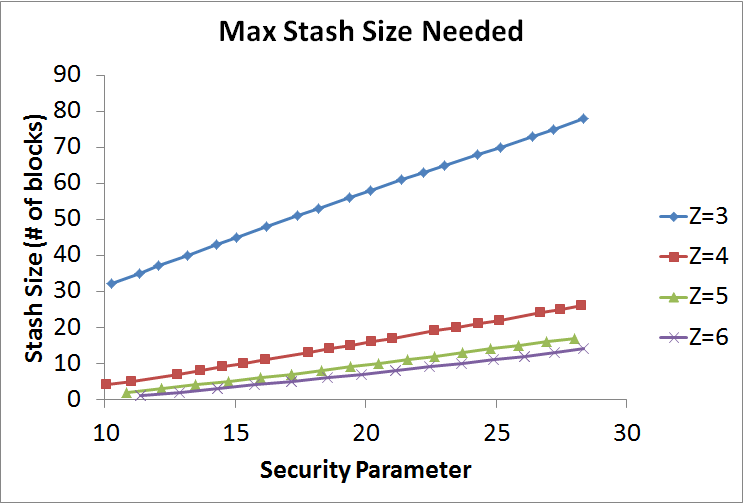
\includegraphics[
				height=5cm,
				keepaspectratio
			]{static/images/max-stash-size-linear.png}
				
		\end{figure}
		
	\end{center}

	Figure 3 from~\cite{Stefanov:2013:POE:2508859.2516660}.

\end{frame}

\begin{frame}{Max stash size for large security parameters}
	
	\begin{center}

		\begin{figure}\manuallabel{tbl:stash-size-for-sec-parameters}{table}

			\begin{tabular}{ l c c c }

				\toprule%

				\multirow{3}{*}{\textbf{Security parameter} $\lambda$}	& \multicolumn{3}{c}{\textbf{Bucket size} $Z$}					\\
																		& 4												& 5		& 6		\\
																		& \multicolumn{3}{c}{\textbf{Max stash size}}					\\

				\midrule%

				80														& 89											& 63	& 53	\\
				128														& 147											& 105	& 89	\\
				256														& 303											& 218	& 186	\\

				\bottomrule%

			\end{tabular}

		\end{figure}

	\end{center}

	Figure 5 from~\cite{Stefanov:2013:POE:2508859.2516660}.

\end{frame}

\begin{frame}{Max stash size does not depend on $N$}
	
	\begin{center}

		\begin{figure}\manuallabel{fig:stash-size-does-not-depend-on-n}{figure}

			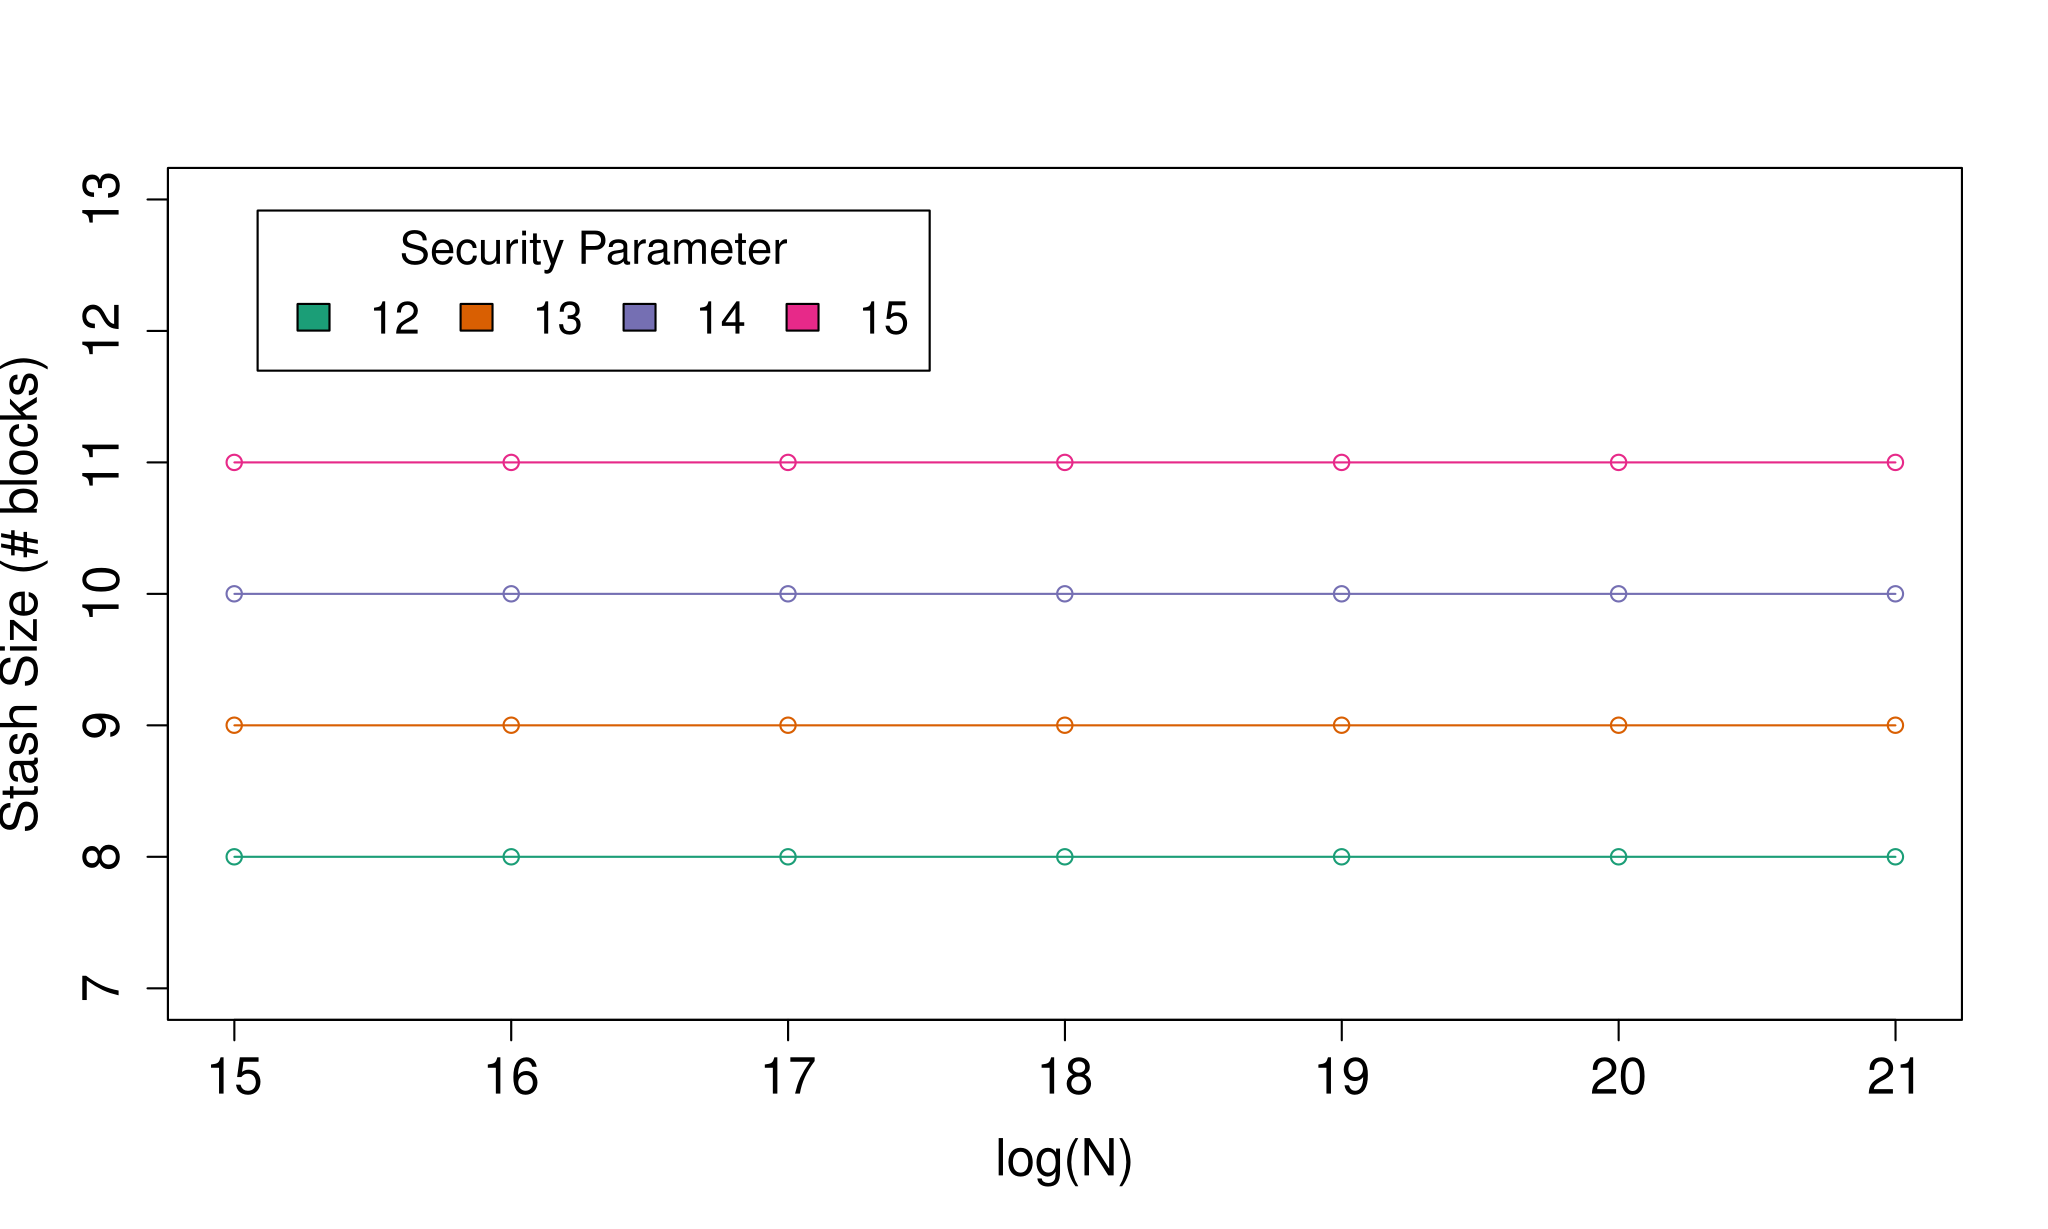
\includegraphics[
				height=5cm,
				keepaspectratio
			]{static/images/stash-size-does-not-depend-on-n.png}

		\end{figure}

	\end{center}

	Figure 4 from~\cite{Stefanov:2013:POE:2508859.2516660}.

\end{frame}

	
\end{document}
